\newpage
\stepcounter{handout}

\begin{exercisebox}[adjusted title= Introduction to Lists and For Loops]
With \ttpy{for loops}, we can avoid duplicated code and iteratively operate, such as drawing 3 circles on a screen.
Start a new project and insert the following code:

\begin{lstlisting}[language=JavaScript]
// Initialize Lists

// List of x-coordinates for the circles
let xs = [30, 50, 70, 90, 110, 130];
// List of y-coordinates for the circles
let ys = [30, 50, 70, 90, 110, 130];

function setup() {
  // Create a canvas with a width and height of 400 pixels
  createCanvas(400, 400);
  // Set the background color to black
  background(0);
}

function drawCircle(x, y) {
  // Disable the outline (stroke) for the circles
  noStroke();
  // Generate a random red color value between 0 and 255
  bubble_R = random(256);
  // Generate a random green color value between 0 and 255
  bubble_G = random(256);
  // Generate a random blue color value between 0 and 255
  bubble_B = random(256);
  // Set the fill color using the random RGB values
  fill(bubble_R, bubble_G, bubble_B);
  // Draw a circle at the specified (x, y) coordinates
  circle(x, y, 25);
}

function draw() {
  // Call the drawCircle function for each pair of (x, y) coordinates
  for (var i = 0; i < xs.length; i++) {
    drawCircle(xs[i], ys[i]);
  }
}
\end{lstlisting}
\end{exercisebox}

\begin{exercisebox}[adjusted title= Explanation Loops I ]
What happens when you run the code? Explain here how a loop produces the result, and give yourself time to understand the logic. This code draws multiple circles on a black background at predefined positions. Each circle is filled with a random color, and the process repeats every frame (due to the \texttt{draw()} function), although the positions and colors remain constant unless the \texttt{xs} or \texttt{ys} arrays are changed dynamically during execution.

\begin{enumerate}
    \item \textbf{Global Variables:}
    \begin{itemize}
        \item \texttt{xs} and \texttt{ys} are arrays (lists) that store the x and y coordinates for the circles. Each pair of values from these arrays will be used to draw a circle on the canvas.
    \end{itemize}

    \item \textbf{setup() Function:}
    \begin{itemize}
        \item The \texttt{setup()} function is called once when the program starts. It creates a canvas of 400x400 pixels and sets the background color to black.
    \end{itemize}

    \item \textbf{drawCircle(x, y) Function:}
    \begin{itemize}
        \item This is a custom function designed to draw a single circle at the specified (x, y) coordinates.
        \item Inside this function:
        \begin{itemize}
            \item \texttt{noStroke()} is called to ensure the circles don't have an outline.
            \item \texttt{random(256)} is used to generate random values for the red (\texttt{bubble\_R}), green (\texttt{bubble\_G}), and blue (\texttt{bubble\_B}) color components, resulting in a random color.
            \item \texttt{fill(bubble\_R, bubble\_G, bubble\_B)} sets the fill color for the circle using the randomly generated RGB values.
            \item \texttt{circle(x, y, 25)} draws a circle at the specified coordinates with a diameter of 25 pixels.
        \end{itemize}
    \end{itemize}

    \item \textbf{draw() Function:}
    \begin{itemize}
        \item The \texttt{draw()} function is called repeatedly, continuously executing the code within it.
        \item Inside \texttt{draw()}, a \texttt{for} loop iterates over the \texttt{xs} array. For each iteration, it retrieves the corresponding x and y coordinates from \texttt{xs} and \texttt{ys} arrays and passes them to the \texttt{drawCircle()} function to draw a circle.
        \item As a result, a set of circles is drawn on the canvas at the specified coordinates, each with a random color.
    \end{itemize}
\end{enumerate}
\end{exercisebox}






\begin{exercisebox}[adjusted title= More with Lists and For Loops II]
The following code snippet has a few changes: We now use a loop to generate our list! Paste the code into a new project and consider the differences in the various loops.

\begin{lstlisting}[language=JavaScript]
// Initialize Lists
// Empty array to hold x-coordinates for the circles
let circleList = []; 

function setup() {
  createCanvas(400, 400);  
  background(0); 
}

function drawCircle(x, y) {
  noStroke(); 
  // Generate a random  colors value between 0 and 255
  bubble_R = random(255);  
  bubble_G = random(255); 
  bubble_B = random(255);
   // Set the fill color using the random RGB values
  fill(bubble_R, bubble_G, bubble_B); 
  circle(x, 200, 50);  // Draw a circle
}

function createCircleList(n) {
// Add a new x-coordinate to the circleList array, spaced by 60 pixels
  for (var i = 0; i < n; i++) {
    append(circleList, i * 60);    }
}

function draw() {
// Draw a circle at each x-coordinate in the circleList, with y fixed at 200
  createCircleList(10);  // Populate the circleList with 10 x-coordinates
  for (var i = 0; i < circleList.length; i++) {
    drawCircle(circleList[i], 200);  
  }
}
\end{lstlisting}

\noindent


\noindent
\end{exercisebox}


\begin{exercisebox}[adjusted title= Explanation for Loops II]
\begin{itemize}
  \item \textbf{createCircleList(n) Function:}
 
  \begin{itemize}
  \item A loop runs n times, appending new values to circleList.
  \item Each value added is i * 60, where i is the loop counter, resulting in x-coordinates spaced 60 pixels apart.
		
  \end{itemize}
  \item \textbf{draw() Function:}
  \begin{itemize}
  \item createCircleList(10): Calls the createCircleList() function to generate 10 x-coordinates and store them in circleList.
\item	 A loop then iterates over circleList, calling drawCircle() for each x-coordinate, with the y-coordinate fixed at 200 pixels.
\item This results in 10 circles being drawn on the canvas.
  \end{itemize}
  \end{itemize}
\end{exercisebox}

%%%% FSM
%\begin{exercisebox}[adjusted title= Finite state machines]
%
%\begin{minipage}{1.0\linewidth}
%\begin{wrapfigure}[9]{r}{0.15\textwidth}
%   \vspace{-1em}
%   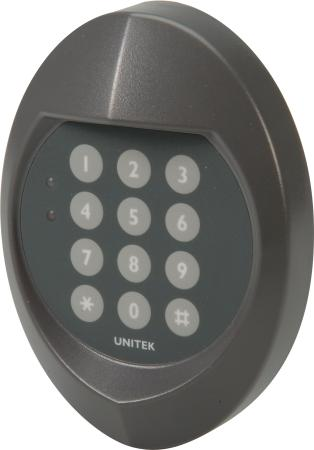
\includegraphics[width=0.15\textwidth]{illustrationer/unitek_kombinationslaas.jpg}
%\end{wrapfigure}
% 
%As the first example of a state machine, we will create one
%electronic combination lock, such as those used for access control
%doors.
%
%\noindent
%Tilstandsdiagram:
%
%\noindent
%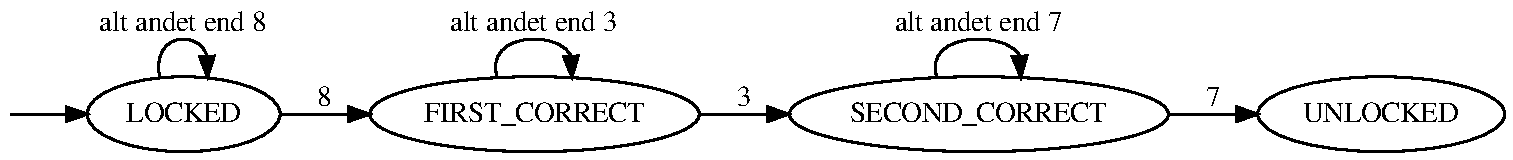
\includegraphics[width=0.85\textwidth]{graphviz/combinationLock_dumb}
%
%%%% FIX!!!!
%Download the Processing.py code for the combination lock here:
%\mbox{\url{http://kortlink.dk/ufdh}} and copy it into a new Processing project.
%
%\end{minipage}
%
%\begin{itemize}
%\item Test the combination lock and watch as the state changes. If you
%did not know the ransom (password), how many attempts does it require?
%to guess?
%
%\item Change the code so that the default is 524 instead
%\item Try changing the code to follow this diagram instead, where incorrect presses reset the state to start:
% 
%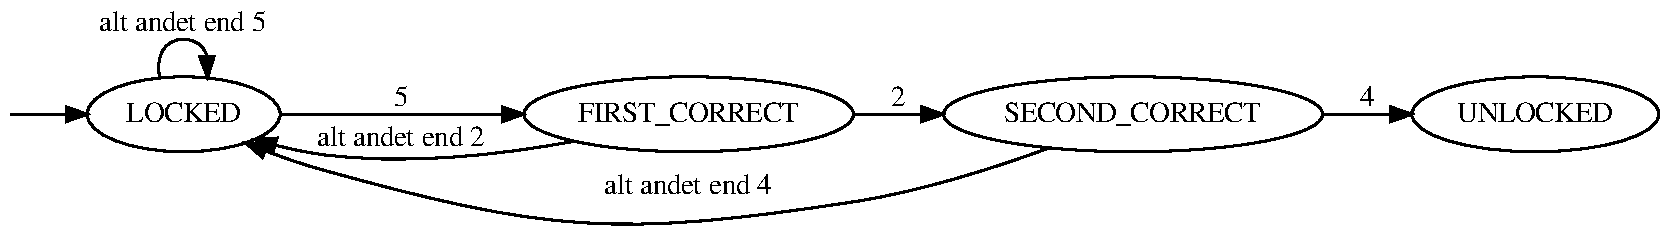
\includegraphics[width=0.85\textwidth]{graphviz/combinationLock_resetting}
%
%\item Draw an extended state diagram of the combination lock with an extra mode, so 4 digits are required. Next, add the extra state in the code.
%\end{itemize}
%\end{exercisebox}
%
%\begin{exercisebox}[adjusted title= Automatic relock after 2 seconds]
%
%Let's extend the lock so that the door automatically locks again after 2 seconds,
%which corresponds to 120 frames:
%
%\noindent
%\begin{center}
%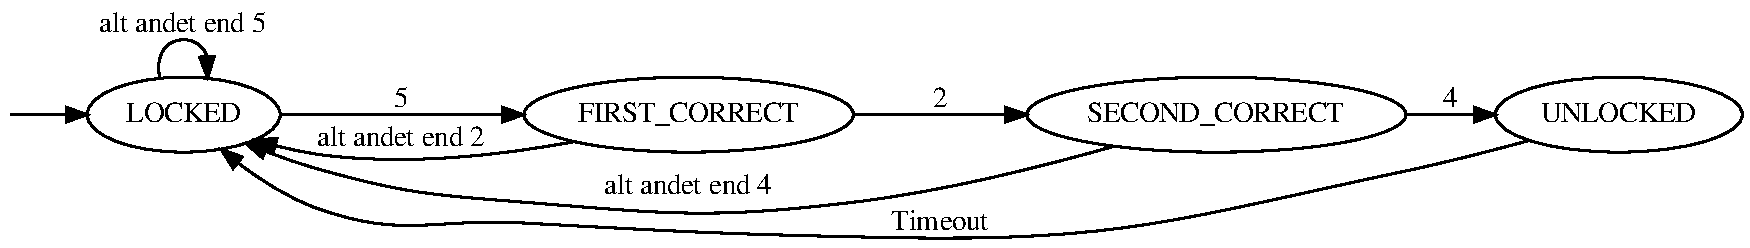
\includegraphics[width=1.0\textwidth]{graphviz/combinationLock_timeout}
%\end{center}
%
%\begin{itemize}
%\item Create a global variable ``\ttpy{timer}'' and set it to 0
%\item Set the \ttpy{timer} variable to 120 as soon as the lock is unlocked, it will
% say when it changes \ttpy{lockState} to \ttpy{"UNLOCKED"}.
%\item Count down with the timer in each frame (add the following to the \ttpy{draw} function):
%
%
%\begin{python}
%global timer
%if timer > 0:
%   timer = timer - 1
%\end{python}
%\item Når timeren er talt helt ned, skal låsen åbnes. I
% \ttpy{draw}-funktionen skal I nu tjekke om vi er i tilstanden
% \ttpy{"UNLOCKED"} og timeren samtidig er talt ned til 0. Indsæt
% følgende i \ttpy{draw}:
% 
%\begin{python}
%if lockState == "UNLOCKED":
%   if timer == 0:
%       lockState = "LOCKED"
%\end{python}
%
%\end{itemize}
%\end{exercisebox}
